%=========================================================================
% (c) Radim Loskot, 2014

\chapter{Úvod}
\label{Chapter.Introducion}
Úvodní text.

\chapter{Renderovací stroj CSSBox}
\label{Chapter.CSSBox}

\chapter{Analýza podpory skriptování v jazyce Javascript v Javě}
\label{Chapter.JavaScriptInJavaAnalysis}

Tato kapitola se zabývá analýzou skriptování a nástrojů, které lze využít pro tvorbu skriptů. Zaměřuje se skriptovací jazyk JavaScript a jeho použití v Javovských aplikacích. Kapitola záměrně popisuje zejména skriptovací engine Rhino a na standardní skriptovací Java API, jež lze pro skriptování použít.

Skriptovací jazyky jsou programovací jazyky, které nám umožňují psát tzv. skripty. Na rozdíl od kompilovatelných zdrojových kódů, je kód skriptu vyhodnocován a interpretován tzv. virtuálním strojem – za běhu skriptu. Většina skriptovacích jazyků je typována dynamicky za běhu skriptu, což nám umožnuje vytvářet proměnné bez specifikace typu, jelikož typová konverze je prováděna automaticky. V dynamických jazycích můžeme použít jednu proměnnou pro uložení více typů. Skriptovací jazyky mají jednoduchou syntaxi, což umožňuje v určitých případech vyřešit poměrně složité problémy pomocí relativně krátkého kódu, efektivně a poměrně v krátkém čase.

Ačkoliv jsou skripty obvykle kompilovány za běhu skriptu, lze je zkompilovat do bajtkódu Javy a nechat je vykonat JVM\footnote{JVM  (Java Virtual Machine) -- virtuální stroj Javy zpracovávající mezikód jazyka Java (Java bytecode)}. V Javě bylo implementováno mnoho skriptovacích Jazyků, využívajících různá rozhraní pro skriptování, což bylo mj. i důvodem pro vznik obecného skriptovacího Java API (viz kapitola XY). Mezi nejrozšířenější skriptovací jazyky pro Javu můžeme zařadit BeanShell, s velmi podobnou syntaxí jakou disponuje Java, a další implementace již existujících jazyků v Javě jako je např. Jython – implemetance Pythonu,  JRuby – implementace Ruby, Groovy aj.

Interpretů JavaScriptu implementovaných v Javě běžících na JVM není mnoho. Z důvodu výkonnosti je většina interpretů Javascriptu pro webové prohlížeče napsána nativně v C nebo C++ a využívá JIT\footnote{JIT (Just in Time) -- metoda překladu urychlující běh skriptu překladem kódu do strojového jazyka} techniky. Jmenovitě nejznámější nativní javasriptová jádra jsou z rodiny „Monkey“, kterou spravuje společnost Mozilla, a která jsou postupně využívána ve webovém prohlížeči Firefox. Dalšími jádry ostatních webových prohlížečů je V8 použité v Google Chrome, Carakan v Opeře, Chakra v Iternet Exploreru nebo JavaScriptCore v prohlížeči Safari.

Nejznámější interprety cílené pro Java aplikace máme v současnosti pouze tři. Nejznámějším interpretem je již zmíněné Rhino (kapitola XY) (10), který je i dodáván jako výchozí skriptovací jazyk v Oracle implementaci JDK 6 a 7\footnote{JDK (Java Development Kit) -- balík základních nástrojů potřebných pro vývoj aplikací pro platformu Java}. Dalším a s velkým budoucím potenciálem je stále ve vývoji interpret Nashorn (kapitola XY) (7), který bude součásti Oracle implementace JDK 8. Oba zmíněné skriptovací jazyky implementují standardní skriptovací Java API (kapitola XY). Rhino bylo o skriptovací API rozšířeno firmou Sun, kdežto Nashorn je vyvíjen s tím API zprvu počátku. Posledním a nepříliš používaným interpretem je YAJI (9), který se snaží oživit starý interpret FESI (8), tím že do něho přidává většinu vlastností z nejnovější specifikace ECMAScriptu.

\section{Rhino}
\label{Chapter.JavaScriptInJavaAnalysis.Rhino}

Rhino je implementace javasriptového jádra napsaná v programovacím jazyce Java. Projekt Rhina byl zahájen v roce 1997 firmou Netscape, kdy firma potřebovala integrovat podporu Javascriptu do budoucího prohlížeče založeném na platformě Java. Rhino vzniklo portem nativní knihovny SpiderMonkey, takže i nyní si lze v kódu nevšimnout Javovských ekvivalentů nepodmíněných skoků. (2)

Projekt prohlížeče, tzv. Javagatoru, byl ovšem velmi brzy pozastaven a Rhino zůstalo dále jen velmi pozvolna vyvíjené několika vlastníky, včetně společnosti Sun. V roce 1998 bylo Rhino uvolněno společnosti Mozilla a držitelé licencí se dohodli, že vydají Rhino jako svobodný software. Nyní je Rhino spravováno pod křídly Mozilly. (2)

\subsection{Vlastnosti Rhina}
\label{Chapter.JavaScriptInJavaAnalysis.Rhino.RhinoFeatures}

V současnosti je vydáno Rhino s označením 1.7R4. Nejnovější verze implementuje všechny vlastnosti Javasriptu 1.7, tzn. je plně ekvivalentní s 3. vydáním standardu ECMA-262 ECMAScript a přidává některé nové vlastnosti, jako jsou doplňky pro práci s poli a podpora E4X\footnote{Rozšíření programovacího jazyka ECMAScript, které přidává podporu nativního XML a vychází z normy ECMA-357 ECMAScript pro XML.}. Od verze 1.7R3 Rhino přidává i částečnou podporu Javasriptu 1.8 a 5. vydání ECMAScriptu, která byla nejnovější verzi 1.7R4 zejména optimalizována a jen mírně rozšířena. (3) (4)

Významnou předností Rhina je jeho dobrá provázanost s Javou, což umožňuje z kódu Javascriptu volat jakýkoliv konstruktor nebo metodu definovanou v Javě. Dosaženo je toho pomocí objektového adaptéru – speciální třídou \texttt{JavaAdapter}. Adaptér vytváří pomocí reflexe objekty Javy a implementuje do objektů navíc metody rozhraní Scriptable, čímž zpřístupňuje tyto objekty pro přímé použití ve skriptech Javascriptu. Adaptér můžeme buď přímo zavolat nebo nechat Rhino ho nechat automaticky odvodit (kód \ref{Algorithm.JavaAdapterInRhino}). 

\begin{table}[ht] 
    \texttt{\begin{tabbing}
      	{ }{ }{ }{ }{ }\={ }{ }\=\+\kill
      	// přímé zavolání adaptéru \\
      	\textbf{var} arr1 = \textbf{new} JavaAdapter(java.util.ArrayList, {}); \\
		// automatické odvození – Rhino zavolá adaptér automaticky \\
		\textbf{var} arr2 = \textbf{new} java.util.ArrayList();
    \end{tabbing}}
\end{table}
\vspace{-12mm}
\begin{algoritmus}
	\caption{Demonstrace explicitního a implicitního volání adaptéru Javy}
	\label{Algorithm.JavaAdapterInRhino}
\end{algoritmus}

Mezi další přednosti Rhina patří možnost rozdělení skriptů do modulů, tak jak bylo specifikováno skupinou CommonJS\footnote{CommonJS – Skupina lidí snažící se vytvořit jednotné Javascriptového prostředí pro servery, desktopy a prohlížeče.} a možnost vysledovat zdroj odkud skript pochází a zpracovávat skript podle odpovídající bezpečnostní politiky. Bezpečnostní politiky v Rhinu vycházejí z Netscape Navigatoru a jejich aplikace je založená na kontrole URL zdroje. (5)

Rhino umožňuje dva režimy – interaktivní a kompilovaný. V kompilovaném módu je kód přeložen do bajtkódu Javy a interpretován dále v JVM. V interaktivním módu je skript spouštěn jednoduchým interpretem, aniž by docházelo ke generování bajtkódu Javy.

\subsection{Skriptování s Rhinem}
\label{Chapter.JavaScriptInJavaAnalysis.Rhino.ScriptingWithRhino}

Zdrojové kódy Rhina jsou strukturovány do několika hlavních balíků, pro konstrukci skriptů v Javě ale využijeme hlavně veřejné API z balíku org.mozilla.javascript.

Základním prvkem pro spuštění jakéhokoliv skriptu je objekt třídy Context, jenž nese vláknově specifické informace o prostředí pro běh skriptů. Každé programové vlákno, které vyžaduje spuštění skriptu, by si mělo asociovat vlastní kontext zavoláním \texttt{Context.enter()} a uvolnit zavoláním \texttt{Context.exit()}. (7)

Úložiště pro objekty nejvyšší úrovně nazýváme v Javascriptu jako tzv. scope. Do scopu vkládáme všechny vlastní objekty, Scope představuje jakousi množinu objektů. Objekt scopu je v Rhinu klasický Javascriptový objekt, který implementuje třídu Scriptable a který by měl obsahovat základní stadardní objekty \texttt{Object} a \texttt{Function}. Inicializovaný scope můžeme získat zavoláním metody \texttt{initStandardObjects} objektu kontextu. Důležitou vlastností scopu je, že scope je kontextově nezávislý, i přestože scope může být vytvořen z kontextu. Scope vytvořený jedním kontextem můžeme vyhodnotit s využitím jiného kontextu. Ve vícevláknových aplikacích lze nechat jeden scope vyhodnotit více odlišnými kontexty zároveň. Rhino zajištuje, že přístup k vlastnostem objektu je atomický. (7)

Objekty Javy, které chceme zpřístupnit do kódu skriptu by měly implementovat rozhraní \texttt{Scriptable} a poskytnout metody pro práci s vlastnostmi objektu: \texttt{get()}, \texttt{put()}, \texttt{has()} a \texttt{delete()}. Základní implementaci rozhraní \texttt{Scriptable} a přístup k atributům objektu pomocí hashovací tabulky poskytuje v Rhinu třída \texttt{ScriptableObject}. Kromě toho třída \texttt{ScriptableObject} implementuje některé důležité metody pro definování hostovaných objektů z tříd Javy, jako je např. statická metoda \texttt{defineClass()}.

Posledním důležitým rozhraní je rozhraní \texttt{Function}. které je implementováno všemi funkčními objekty Javasriptu. Pokud chceme funkci zavolat, můžeme k tomu použít metody \texttt{call()} nebo \texttt{construct()} v závislosti na tom, jestli funkce má být volání s klíčovým slovem \texttt{new}.

Javascript kromě základního objektu Object, který musí v Javě implementovat již zmíněné rozhraní \texttt{Scriptable}, obsahuje i 5 primitivních datových typů. Tyto datové typy musí být mapovány do Javy na odpovídající třídy. Jakým způsobem je mapování docíleno, je znázorněné v tabulce \ref{Table.JavaScriptToJavaMapping}. 

\begin{table}[H]
  \begin{center} 
    \begin{tabular}{| c | l |} \hline
    \textbf{Typ v Javascriptu} & \textbf{Reprezentace v Javě} \\ \hline
    Undefined & org.mozilla.javascript.Undefined \\ \hline
    Null & null \\ \hline
    Boolean & java.lang.Boolean  \\ \hline
    Number & java.lang.Number \\ \hline
    String & java.lang.String \\ \hline
    \end{tabular}
    \caption{Mapování primitivních typů Javascriptu do Javy (11)}
    \label{Table.JavaScriptToJavaMapping}
  \end{center}
\end{table}

\subsection{Princip kompilátoru a interpretu}
\label{Chapter.JavaScriptInJavaAnalysis.Rhino.CompilerTechniques}

V předchozí kapitole jsme zmínili sadu nejdůležitějších tříd a rozhraní z veřejného API Rhina. V balíku \texttt{org.mozilla.javascript} se ovšem nachází i jednotlivé části zajišťující samotnou funkci překladače a interpretu Javascriptu.

Mezi nejpodstatnější neveřejné třídy v balíku patří např. třída \texttt{ScriptRuntime} obsahující metody využívané interpretem a optimalizátorem jazyka pro generování bajtkódu Javy. Formát bajtkódu lze konkrétně nalézt v balíku \texttt{src.org.mozilla.classfile}. Překlad Javascriptu do bajkódu probíhá běžně za běhu programu. Explicitní překlad skriptu a vytvoření .class souboru lze vynutit zavoláním překladače Javascriptu, příkazem:

\centerline{\texttt{java org.mozilla.javascript.tools.jsc.Main script.js}}

Vlastní překladač do bajkódu Javy je velkým specifikem Rhina. Pro každý zkompilovaný skript je vygenerována přesně jedna odpovídající třída v Javě, která implementuje rozhraní Script. Skript lze potom vykonat zavoláním metody \texttt{exec()} rozhraní Script.

Interaktivní (nekompilovaný) režim interpretu Javascriptu zajišťuje třída \texttt{Interpret}, která je umístěná také v hlavním balíku. Interpret JavaScriptu v Rhinu je klasický zásobníkový automat. Pro reprezentaci mezikódu se používá instrukce s proměnlivou délkou. Instrukce se skládá z operačního kódu a případných operandů. Prováděcí smyčku interpretu implementuje metoda \texttt{interpretLoop()}, která přijímá aktuální rámec volání a kontext, ve kterém interpretování probíhá. Rámec volání obsahuje typické položky jako zásobník hodnot, pole symbolů a aktuální scope objekt.

Zajímavostí je zavedení v interpretu dvou druhů zásobníků – hlavního a číslicového. Hlavní zásobník je určen pro obecné hodnoty, tzn. pro hodnoty všech typů JavaScriptu. Číslicový zásobník slouží pro uložení hodnot JavaScriptového primitivního typu Number. Hlavní zásobník je implementován v Javě jako pole objektů Object a číslicový jako pole primitivního typu double. Mezi hlavním a číselným zásobníkem probíhá mapování. Pokud je v hlavním zásobníku uložená unikátní hodnota \texttt{DBL\_MRK}, tak bude čtení odpovídající hodnot pokračovat ve druhém zásobníku (viz obrázek \ref{Figure.RhinoStack}). Tato technika byla zavedena čistě z důvodu optimalizace, aby nedocházelo ke zbytečnému \csuv{zabalení} primitivního typu do objektu, aby se šetřila alokace paměti pro objekt a příp. dereference ukazatelů.

\begin{figure}[H]
  \begin{center}
    \scalebox{0.40}{
      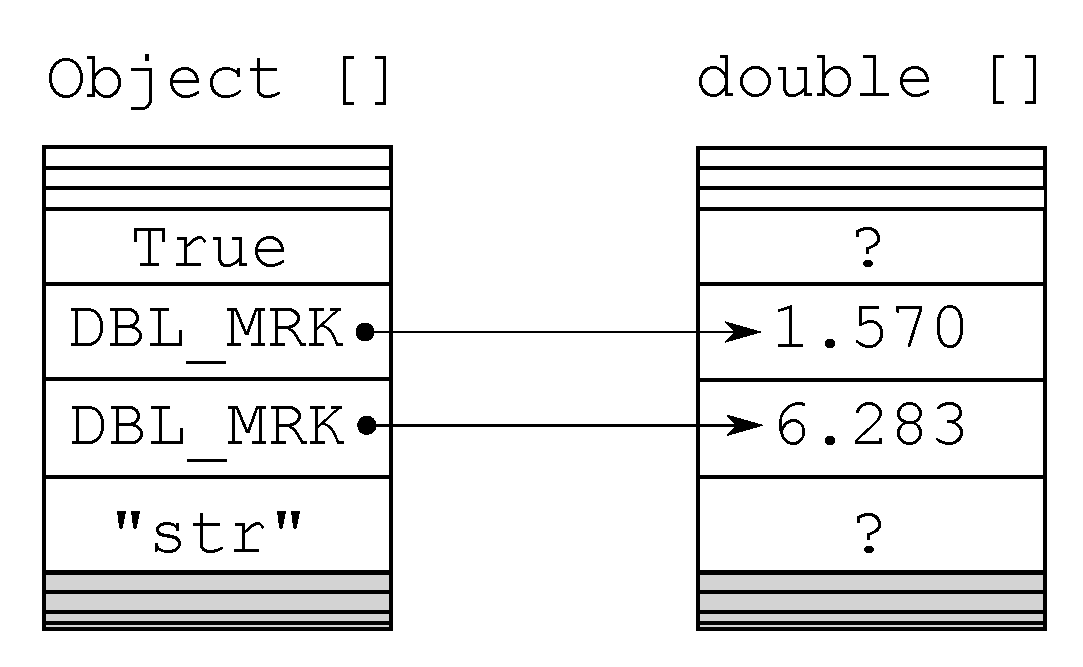
\includegraphics{fig/rhino_stack.pdf}
    }
    \caption{Znázornění koexistence hlavního a číslicového zásobníku}
    \label{Figure.RhinoStack}
  \end{center}
\end{figure}

Interpret JavaScriptu přijímá mezikód jazyka, který je generován metodou compile třídy \texttt{CodeGenerator}. Generátor mezikódu pracuje s abstraktním syntaktickým stromem tvořeným z prvků definovaných v balíku \texttt{org.mozilla.javascript.ast} a generovaným třídou \texttt{Parser}.

\section{Nashorn}
\label{Chapter.JavaScriptInJavaAnalysis.Nashorn}

Nashorn je projekt, který si klade za cíl vyvinout zcela nový, odlehčený a výkonný Javascriptový runtime pro nativní JVM. Výstupem projektu by měla být schopnost spouštět Javascriptový kód příkazem jrunscript, která podléhá specifikaci JSR 223\footnote{JSR 223 -- specifikace definující framework pro vkládání skriptů do zdrojového kódu Javy}. Oproti poměrně letitému Javascriptovému interpretu Rhina vyvinutému pro tehdejší JVM, se Nashorn zaměřuje na nové techniky používání dynamických jazyků v Javě a vychází ze specifikace tzv. Da Vinci stroje (JSR 292\footnote{JSR 292 -- specifikace pro rozšíření JVM o nativní podporu dynamických jazyků}). (6)

Jádro interpretu Nashorn vychází z ECMAScriptu verze 5.1. Skripty jazyka Javascript lze v Javě vytvářet užitím klasického Java API pro skriptování popsaného blíže v kapitole \ref{Chapter.JavaScriptInJavaAnalysis.ScriptingJavaAPI}. Konkrétně instanci Javascriptového jádra ScriptEngine získáme vyhledáním odpovídajícího slova např. „nashorn“ v továrně ScriptEngineManager. Naopak pokud chceme spustit Javascriptový skript můžeme toho dosáhnout příkazem jrunscript a specifikací skriptovacího jazyka přepínačem \texttt{-l}, předáním skriptu přepínačem \texttt{-e}, nebo souboru se skriptem přepínačem \texttt{-f}.

\section{Skriptovací Java API}
\label{Chapter.JavaScriptInJavaAnalysis.ScriptingJavaAPI}

V Javě byly postupem času implementovány všechny nejznámější skriptovací jazyky používající různá a vlastní rozhraní. To bylo základním podmětem pro vytvoření obecného a přenositelného skriptovacího Java API, které umožňuje propojit skripty s aplikací Javy. API muselo být napsáno velmi abstraktně, aby bylo aplikovatelné na jakýkoliv rozmanitý skriptovací engine, ale zároveň muselo zahrnout všechny specifické aspekty známých skriptovacích jazyků. (12)

Skriptovací Java API vychází ze specifikace JSR 223. Specifikace definuje standardní framework a API pro tvorbu skriptu a jejich vkládání jich do Javovských aplikací. Specifikace ovšem nedefinuje jaký jazyk pro skriptování musíme zvolit, proto můžeme použít pro skriptování jakýkoliv jazyk, který je kompatibilní s JSR 223. Použitím standardního API, máme možnost psát skripty kompatibilní s JSR 223 (kapitola XY). A naopak při psaní skriptu, který je kompatibilní s JSR 223, máme garantováno, že budeme mít přístup k jakékoliv standardní Java knihovně.

Implementace Java API v JDK od Oraclu vychází z frameworku BSF (13). Tento framework byl vyvinut firmou IBM a ve verzi 2.x poskytoval základní množinu tříd umožňujících podporu skriptovacích jazyků v aplikacích Javy. S příchodem skriptovacího Java API byl vydán BSF framework verze 3.x, který se poté stal součástí zmíněného JDK.

Základní Oracle implementace JDK 6 a 7 skriptovacího API obsahuje upravený již zmíněný JavaScriptový stroj vycházející z knihovny Rhina. Zahrnutá Oracle verze knihovny Rhina byla omezena o některé vlastnosti, které by poskytovalo přímé použití knihovny. Z důvodu bezpečnosti byl zakázán kompilátor do mezikódu Javy. V JDK nelze najít ani pomocné nástroje příkazové řádky distribuované Rhinem od Mozilly, jako jsou např.: JavaScriptový shell, debugger apod. Použitá implementace Rhina umožňovala definovat abstraktní třídy a implementovat vícenásobná rozhraní pomocí adaptéru JavaAdapter. Oracle nahradil tento adaptér vlastní třídou, která umožňuje implementaci pouze jednoduchých rozhraní. 

\subsection{Architektura skriptování}
\label{Chapter.JavaScriptInJavaAnalysis.ScriptingJavaAPI.ArchitectureOfScripting}

\bigskip \noindent Skriptovací API je umístěné v balíčku \texttt{javax.script}. Skriptování je poměrně přímočaré, abychom mohli začít psát skripty, vždycky musíme nejprve:

\begin{enumerate}
  \item Vytvořit objekt třídy \texttt{ScriptEngineMager} -- Objekt vyhledává skriptovací enginy \texttt{ScriptEngine} v načtených JAR knihovnách, je to tzv. továrna na skriptovací enginy;
  \item Získat instanci skriptovacího enginu \texttt{ScriptEngine} -- Instance skriptovacího enginu je získána z továrny zavoláním např. metody \texttt{getEngineByName()}. 
\end{enumerate}

Jakmile máme získanou instanci skriptovacího enginu, můžeme již vykonávat, definovat, nebo upravovat skripty.

Nejdůležitější metodou rozhraní \texttt{ScriptEngine} je bezpochyby metoda \texttt{eval()}, která nám umožní spouštět skripty. Skript může být předán jako řetězec, nebo může být umístěn v souboru, streamu, či jiné zdroji. V závislosti na tom, zda daný skriptovací jazyk umožnuje vyhodnocování skriptu s výsledkem, tak je metodou \texttt{eval()} navrácen i výsledek skriptu.

Myšlenkou Java API je mít co nejvíce společných rysů skriptovacích jazyků specifikovaných v rozhraní \texttt{ScriptEngine} a nemít zde žádný rys, který by některý skriptovací jazyk nemohl poskytnout. Proto všechny speciální vlastnosti konkrétních skriptovacích jazyků musí být implementovány v odlišných rozhraních. Tento návrh zajišťuje minimum změn těchto rozhraní v budoucnu. Nejdůležitější přídavné rozhraními rozpoznáváme:

\begin{itemize}
  \item \textbf{\texttt{Invocable}} -- Rozhraní implementované enginy, které umožňují volat funkce/metody ve skriptu. Pro volání funkce používáme \texttt{invokeFunction()}, pro metody invokeMethod();
  \item \textbf{\texttt{Compilable}} -- Rozhraní implementované enginy, které jsou schopny kompilovat skript do svého mezikódu.
\end{itemize}

\subsection{Data binding}
\label{Chapter.JavaScriptInJavaAnalysis.ScriptingJavaAPI.DataBinding}

Stěžejním úkolem pro funkci frameworku Java API, je zajistit sdílení dat mezi hostovanou aplikací Javy a skriptovacím enginem. Framework BSF umožňoval sdílení proměnných pouze po náležité registraci v manažeru skriptovacích enginů, k němuž měly přístup všechny skriptovací enginy. Java API jde s modelem dále a udržuje sdílené proměnné pomocí kontextu, ve kterém je skript spouštěn.

Proměnné jsou seskupeny a uloženy ve jmenných prostorech nebo scopech. Abstrakce uchovávání proměnných ve jmenném prostoru (scopu) je dána rozhraním \texttt{javax.script.Bindings}, přičemž se nejedná o nic jiného, než o jednoduché mapování názvu proměnné na náležitý objekt – \texttt{Map<String, Object>}. Každý kontext skriptu obsahuje právě množinu takovýchto jmenných prostorů.

\bigskip \noindent Specifikace uvádí dva základní jmenné prostory:

\begin{itemize}
  \item \textbf{Enginový scope} -- Proměnné, které se vážou k tomuto scopu nejsou viditelné jiným enginem;
  \item \textbf{Globání scope} -- Ke všem proměnným tohoto scopu mají přístup všechny enginy vytvořené danou instancí enginového manažeru.
\end{itemize}

Pokud chceme vytvořit novou proměnou, dosáhneme toho zavoláním metody \texttt{put()} objektu \texttt{Bindings}. Proměnnou v enginovém scopu lze definovat následovně:

\begin{enumerate}
  \item Nastavením vlastního objektu \texttt{Bindings} -- Vytvořit mapovací objekt Bindings, kde vytvoříme naši proměnnou. Tento mapovací objekt nastavíme v enginu buď metodou \texttt{setBindings()}, nebo případně až za běhu skriptu, parametrem v metodě \texttt{eval()};
  \item Využitím enginového objektu \texttt{Bindings} -- Získáme výchozí mapovací objekt enginu metodou \texttt{getBindings()}, do kterého následně vložíme naši proměnou.
\end{enumerate}

Získání hodnoty proměnné se docílí obdobně akorát metodou \texttt{get()}.

Základní vlastností frameworku je uchovávání stavu proměnných po vykonání skriptu. Všechny proměnné, které jsou ve skriptu inicializovány, se také automaticky vloží do odpovídajícího objektu \texttt{Bindings}. Po skončení skriptu nám jsou vytvořené proměnné dostupné v odpovídajícím scopu, kde byly vytvořeny. Tento stav scopu zůstává i do dalšího vyhodnocení metodou \texttt{eval()}.

Jmenné prostory jsou pouze jedním stavebním prvkem další třídy \texttt{SimpleScriptContext} – kontextu skriptu. Všechny stavové objekty, které jsou pro běh skriptu podstatné jsou uložené právě v této třídě. Dokonce i výše popsaný globální a enginový scope je uchováván zde. Jmenné prostory jsou zde uloženy ve formě listu čísel, které identifikují jednotlivé scopy. Čísla ve skutečnosti představují prioritu scopu. Nízká čísla popisují scopy s vysokou prioritou a vysoká čísla s nízkou prioritou. Ve vyhodnocování skriptu to znamená, že pokud např. hledáme proměnou, která je ve dvou scopech zároveň, bude navrácena pouze ta ze scopu, který má vyšší prioritu. Enginovému scopu je přiřazena priorita 100, globálnímu scopu priorita 200. Kromě dvou základních scopů si můžeme definovat i vlastní jmenný prostor. Pro vytvoření vlastního jmenného prostoru ovšem nestačí nastavit tento scope pomocí \texttt{setBindings()} ve třídě \texttt{SimpleScriptContext}, protože třída přijímá pouze dva základní kontexty. Proto musíme definovat svůj vlastní kontext implementující rozhraní \texttt{ScriptContext}.